\section{Resultados}
\label{sec:resultados}

Medimos sobre 14 conjuntos de $10^7$ llaves de 64 bits: cinco reales, seis sintéticos y tres patológicos, en el formato de SOSD~\cite{marcus2020}. Cada estructura respondió $10^6$ consultas aleatorias y
reportamos la mediana de 5 repeticiones del tiempo medio por consulta.

\subsection{P1. ¿Qué tan compacta es la representación?}

\begin{figure}[htbp]
\centering
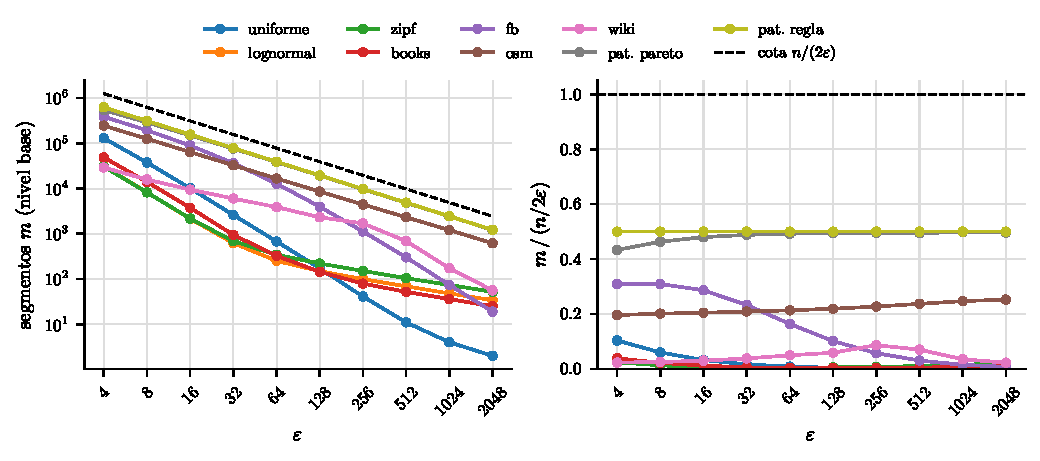
\includegraphics[width=\textwidth]{figuras/segmentos.pdf}
\caption{Izquierda: segmentos del nivel base $m$ según $\varepsilon$, con la cota
$n/(2\varepsilon)$ en línea discontinua. Derecha: $m$ dividido por la cota.}
\label{fig:segmentos}
\end{figure}

\begin{table}[htbp]
\centering\small
\caption{Tamaño del PGM-index con $n=10^7$ y $\varepsilon=64$.}
\label{tab:segmentos}
\begin{tabular}{@{}llrcr@{}}
\toprule
Conjunto & Tipo & Segmentos $m$ & Niveles & Tamaño \\
\midrule
\tabinput{tablas/segmentos.tex}
\bottomrule
\end{tabular}
\end{table}

En todos los conjuntos y para todo $\varepsilon$ se cumple la cota $m\le n/(2\varepsilon)$
(Figura~\ref{fig:segmentos}). En los datos regulares, $m$ queda muy por debajo de ella: con
$\varepsilon=64$, books indexa $10^7$ llaves con 326 segmentos, que ocupan 5\,KB
(Tabla~\ref{tab:segmentos}). Los datos reales más difíciles son osm, fb y friendster, con cerca del
20\,\% de la cota. Los patológicos pareto y regla llegan a la mitad de la cota, que es el peor caso
que observamos. En cambio, loggap, que parece irregular, resulta fácil.

En los datos regulares, $m$ cae más rápido que $1/\varepsilon$ cuando $\varepsilon$ va de 8 a 64,
como predice $m=O(n/\varepsilon^c)$ con $c>1$~\cite{ferragina2020icml}. En osm, wiki y los
patológicos de cola pesada, en cambio, cae a la misma velocidad que $1/\varepsilon$. La recursión
deja índices de 1 a 5 niveles, y construir uno de $10^7$ llaves toma menos de 200\,ms.

\subsection{P2. ¿Cómo influye $\varepsilon$ en el espacio y el tiempo?}

\begin{figure}[htbp]
\centering
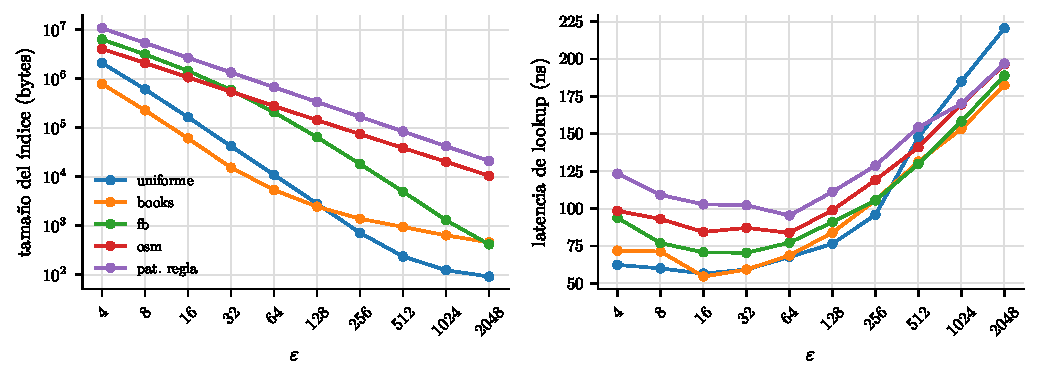
\includegraphics[width=\textwidth]{figuras/epsilon.pdf}
\caption{Efecto de $\varepsilon$ con $n=10^7$: tamaño del índice (izquierda) y tiempo por
consulta (derecha).}
\label{fig:epsilon}
\end{figure}

Al subir $\varepsilon$, el espacio cae varios órdenes de magnitud, pero el tiempo no baja
igual: tiene un mínimo entre $\varepsilon=16$ y $64$ (Figura~\ref{fig:epsilon}). Con
$\varepsilon$ grande domina la búsqueda binaria final sobre la ventana de $2\varepsilon$
llaves, y con $\varepsilon=2048$ el PGM ya no mejora a la búsqueda binaria sobre todo el arreglo
(183 a 221\,ns frente a unos 160\,ns). Con $\varepsilon$ muy pequeño el índice crece y gana niveles sin que la consulta mejore.
En la práctica, un $\varepsilon$ entre 16 y 64 es un buen punto de operación.

\subsection{P3. ¿Cuándo gana frente al B$^+$ tree y la búsqueda binaria?}

\begin{figure}[htbp]
\centering
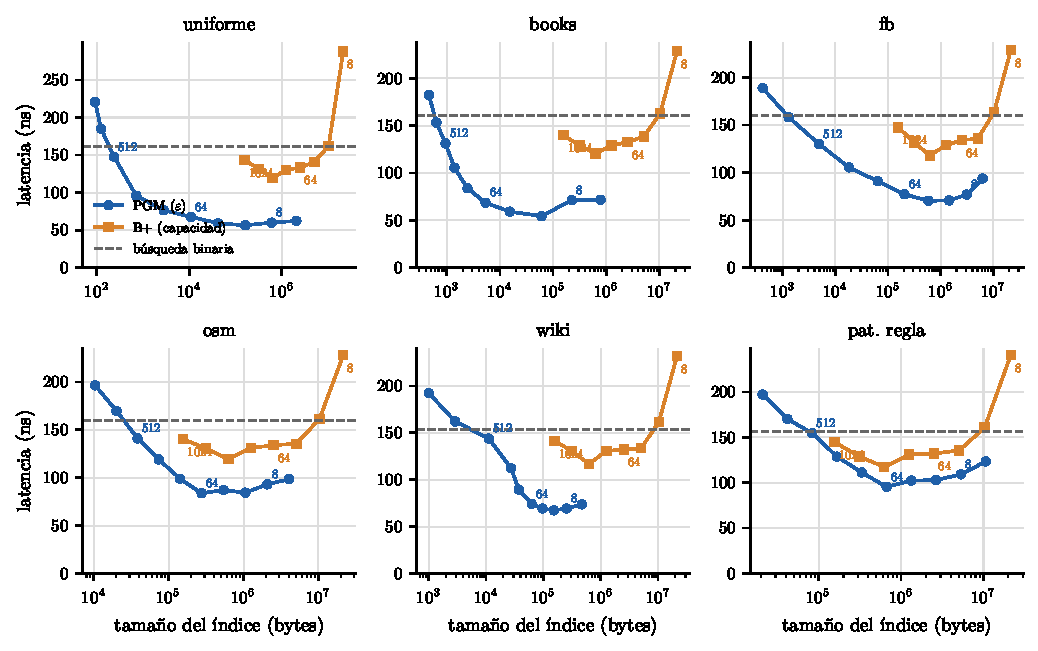
\includegraphics[width=0.85\textwidth]{figuras/pareto.pdf}
\caption{Espacio contra tiempo con $n=10^7$. Cada punto del PGM corresponde a un $\varepsilon$ y cada
punto del B$^+$ a una capacidad de nodo. Más abajo y a la izquierda es mejor.}
\label{fig:pareto}
\end{figure}

\begin{table}[htbp]
\centering\small
\caption{PGM ($\varepsilon=64$), B$^+$ (capacidad 64) y búsqueda binaria con $n=10^7$. El tiempo
es la mediana en ns por consulta.}
\label{tab:comparacion}
\begin{tabular}{@{}lrrrrrr@{}}
\toprule
& \multicolumn{3}{c}{Tiempo (ns)} & \multicolumn{3}{c}{Tamaño del índice} \\
\cmidrule(lr){2-4}\cmidrule(l){5-7}
Conjunto & Binaria & PGM & B$^+$ & PGM & B$^+$ & B$^+$/PGM \\
\midrule
\tabinput{tablas/comparacion.tex}
\bottomrule
\end{tabular}
\end{table}

Con $n=10^7$, el PGM es más rápido y más pequeño que el B$^+$ en los 14 conjuntos
(Figura~\ref{fig:pareto} y Tabla~\ref{tab:comparacion}). Responde en unos 60 a 100\,ns,
frente a unos 130 a 160\,ns del B$^+$ y 150 a 200\,ns de la búsqueda binaria, es decir,
entre 1,4 y 2,3 veces más rápido que el B$^+$ y entre 1,6 y 2,9 veces más rápido que la binaria,
alrededor de dos veces en la mayoría de los conjuntos. En espacio, el B$^+$ ocupa cientos de veces más en los datos
regulares. La ventaja se reduce en los datos más irregulares: en pareto y regla el B$^+$ ocupa
solo 4 veces más, y el mejor PGM es solo 1,2 a 1,3 veces más rápido que el mejor B$^+$.

\begin{figure}[htbp]
\centering
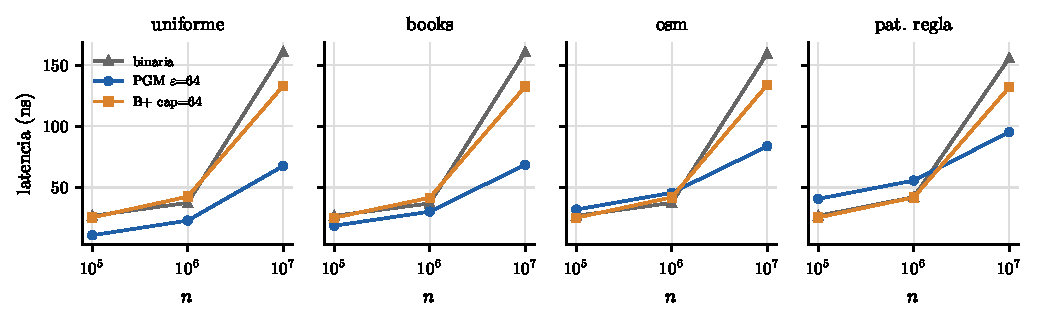
\includegraphics[width=0.85\textwidth]{figuras/tamanos.pdf}
\caption{Tiempo por consulta según $n$, con $\varepsilon=64$ y capacidad 64.}
\label{fig:tamanos}
\end{figure}

El tamaño del arreglo decide cuánto gana el PGM (Figura~\ref{fig:tamanos}). Con $n=10^5$ las
tres estructuras tardan unos 25 a 30\,ns: el PGM gana en los datos regulares,
pero pierde en osm, wiki, zipf, pareto y regla. Con $n=10^7$ las llaves ocupan 80\,MB: la búsqueda
binaria y el B$^+$ dan más pasos sobre el arreglo, mientras que el PGM solo busca dentro de la
ventana final. Ahí el PGM gana en todos los
conjuntos.

\subsection{Versiones dinámicas}
\label{sec:res-dyn}

\begin{figure}[htbp]
\centering
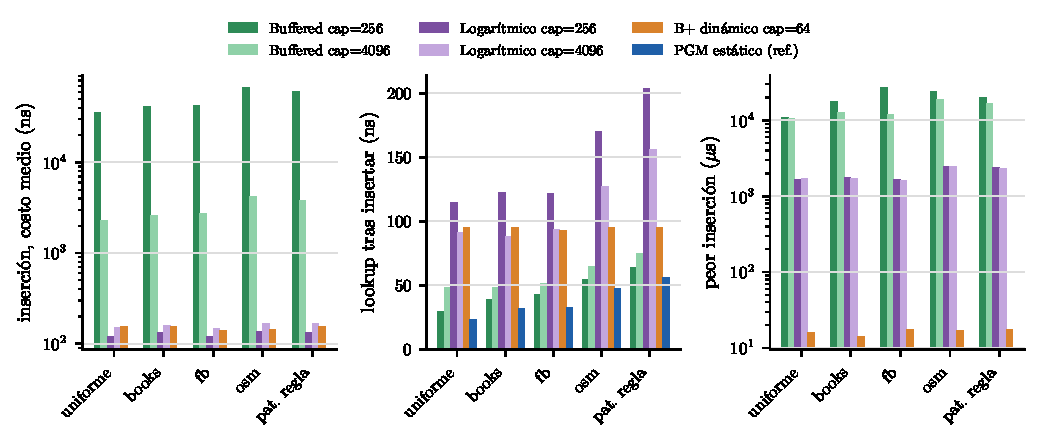
\includegraphics[width=\textwidth]{figuras/dinamicos.pdf}
\caption{Base de $10^6$ llaves más $2\times10^5$ inserciones: costo medio por inserción, tiempo de
búsqueda al terminar e inserción más lenta.}
\label{fig:dinamicos}
\end{figure}

Las dos variantes muestran el compromiso esperado (Figura~\ref{fig:dinamicos}).
\texttt{BufferedPGM} busca algo más lento que el estático (entre 1,3 y 2 veces), y cada
reconstrucción recorre toda la base. Por eso inserta en decenas de microsegundos con buffer 256 y
en unos pocos con buffer 4096, y tiene pausas de decenas de milisegundos.
\texttt{LogarithmicPGM} inserta en 120 a 170\,ns, a la par del B$^+$ dinámico (140 a 155\,ns), y a
cambio busca entre 2 y 4 veces más lento que el estático porque consulta varios niveles. Ambas ocupan casi la mitad de memoria que
el B$^+$ dinámico.
